\documentclass{article}
\usepackage[utf8]{inputenc}
\usepackage{amsmath}
\usepackage{amssymb}
\usepackage{graphicx}
\usepackage{hyperref}
\usepackage{tikz}
\usepackage{pgfplots}
\usepackage{float}
\usepackage{listings}
\usepackage{color}
\usepackage{bbm}
\usepackage{multirow}
\usepackage{comment}

\newcommand{\wb}{\mathbf{w}}
\newcommand{\xb}{\mathbf{x}}

\title{Reinforcement Learning \\ Exercise 7 - Solution}
\author{Jonathan Schnitzler - st166934 \\
Eric Choquet - st160996}
\date{\today}
\begin{document}
\maketitle

\section{Linear function approximation}

\paragraph*{a)  Tabular linear function approximation}

The method of just writing down all values for each state $V(s)$ can be achieved via the identity as a feature vector, also known as one-hot coding, e.g.
\begin{equation}
    x(s_i) = \begin{pmatrix}
        0 & \hdots & 0 & 1 & 0 & \hdots & 0
    \end{pmatrix}^T.
\end{equation}
This results in the same number as features as states in the state space. The tabular value is now just the weight
\begin{equation}
    V(s) = w_i
\end{equation} and the possible non-linear function $f$ is the identity. The state-action value $Q(s, a)$ could be achieved in a similar way, for $x(s, a) = e_j$ and an according enumeration. The linear function approximation
$$\hat{v}(s,w) = \sum_{i=1}^d w_i f(x_i)$$
is a generalization of the tabular methods.

\paragraph*{b) Update rule for Sarsa}

\begin{enumerate}
\item Tabular case
    $$Q(S_t, A_t) \leftarrow Q(S_t, A_t) + \alpha[R_{t+1} + \gamma Q(S_{t+1}, A_{t+1})- Q(S_t, A_t)]$$
    which is equivalent, shown in task a) to
    $$\mathbf{w}_{t+1} = \mathbf{w}_t + \alpha[R_{t+1} + \gamma \hat{q}(S_{t+1},A_{t+1},\mathbf{w})- \hat{q}(S_t, A_t, \wb_t)]$$
    since there $w_{t,i} = Q(s, a)$
\item Function approximation
$$\mathbf{w}_{t+1} = \mathbf{w}_t + \alpha[R_{t+1} + \gamma \hat{q}(S_{t+1},A_{t+1},\mathbf{w})- \hat{q}(S_t, A_t, \wb_t)]\nabla \hat{q}(S_t, A_t, \wb)$$
\item Linear function approximation
$$\mathbf{w}_{t+1} = \mathbf{w}_t + \alpha[R_{t+1} + \gamma \wb^T \xb(S_{t+1},A_{t+1})- \wb^T \xb(S_t, A_t)] \xb(S_{t}, A_t)$$

% \item Tabular case
% $$\sum_{i=q}^d w_i f(s_{t+1}) = \sum_{i=q}^d w_i f(s_t) +\alpha [R_{t+1} + \gamma (\sum_{i=q}^d w_i f(s_{t+1})) - \sum_{i=q}^d w_i f(s_t)]$$
% \item Function approximation
% $$\sum_{i=q}^d w_i x_i(s_t) = \sum_{i=q}^d w_i x_i(s_t) +\alpha [R_{t+1} + \gamma (\sum_{i=q}^d w_i x_i(s_{t+1})) - \sum_{i=q}^d w_i x_i(s_t)]$$
% \item Linear function approximation\\

\end{enumerate}



\section{Mountain Car}

\paragraph*{a) Value Function}

Q-learning uses the update rule
\begin{equation}
    Q(S_t, A_t) \leftarrow Q(S_t, A_t) + \alpha[R_{t+1} + \gamma \max_a Q(S_{t+1}, a) - Q(S_t, A_t)]
\end{equation}

The value function $V(s)$ is defined as the maximum over all possible actions $a$ in state $s$ of the state-action value function $Q(s, a)$. For the Mountain Car problem, we first discretize the state space as suggested in the exercise into 20 by 20 bins of position and velocity, i.e.
\begin{align}
    x_i &= \frac{1.8}{20} \cdot i - 1.2, \quad i = 0, \hdots, 19 \\
    \dot{x}_i &= \frac{0.14}{20} \cdot i - 0.07, \quad i = 0, \hdots, 19
\end{align}
The continuous state space is then rounded to the closest state of this state-aggregation. With three possible actions the state-action value function $Q(s, a)$ is a 20 by 20 by 3 matrix. 

For the tabular version of linear function approximation, the weight vector $\wb$ has the same size and is flatted to 1200 dimensions. The results of the value function during training are depicted in Figure \ref{fig:V1} till Figure \ref{fig:V3}.

\begin{figure}[H]
    \centering
    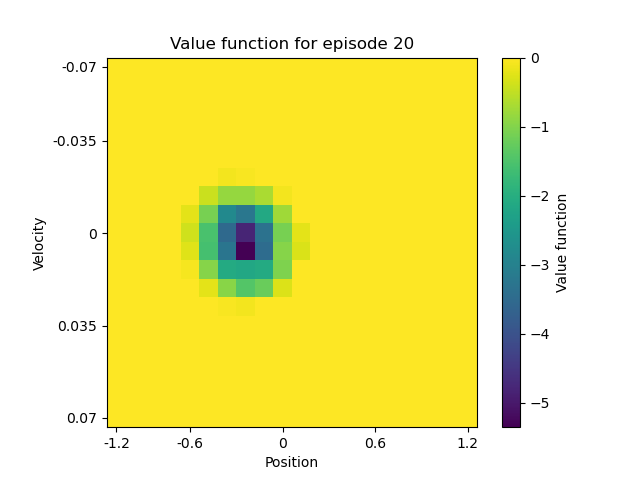
\includegraphics[width=0.8\textwidth]{images/document/value_function_episode20.png}
    \caption{Value function after 20 episodes}
    \label{fig:V1}
\end{figure}

\begin{figure}[H]
    \centering
    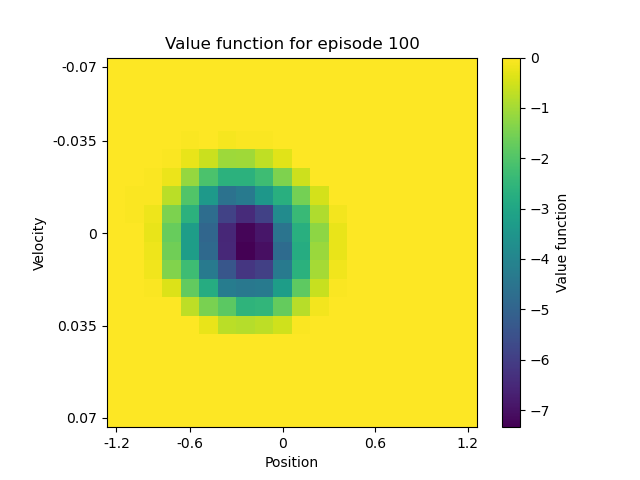
\includegraphics[width=0.8\textwidth]{images/document/value_function_episode100.png}
    \caption{Value function after 100 episodes}
    \label{fig:V2}
\end{figure}

\begin{figure}[H]
    \centering
    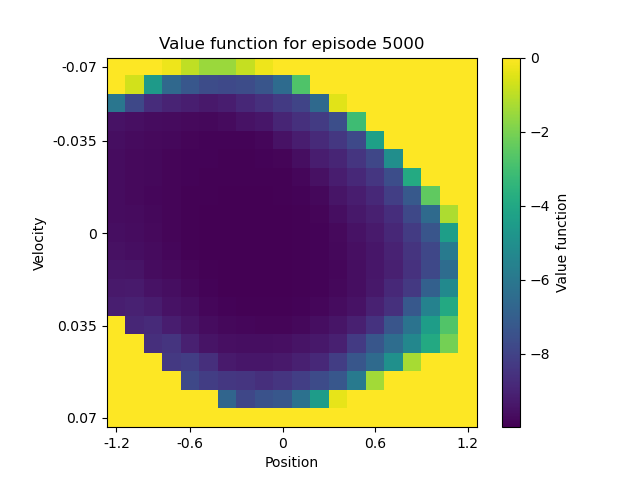
\includegraphics[width=0.8\textwidth]{images/document/value_function_episode5000.png}
    \caption{Value function after 5000 episodes}
    \label{fig:V3}
\end{figure}



\paragraph*{b) Average investigation}

In order to investigate the average performance of the agent, we run the algorithm 10 times and plot the average length and successes per episode. The results are depicted in Figure \ref{fig:average}.

\begin{figure}[H]
\centering
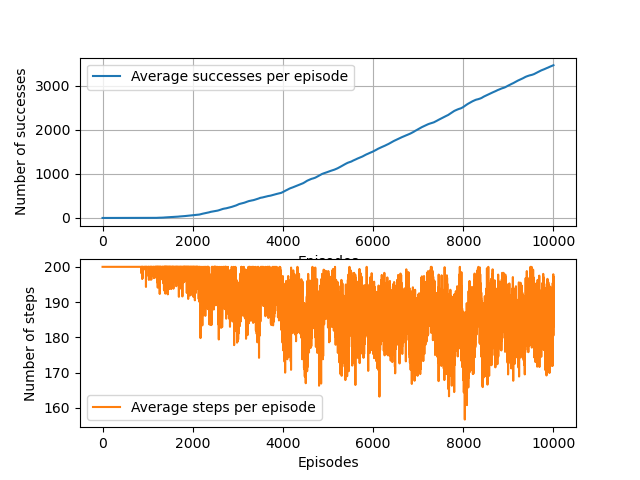
\includegraphics[width=0.8\textwidth]{images/document/repeated_training_investigation.png}
\caption{Averaged evaluation of 10.000 episodes over 10 runs}
\label{fig:average}
\end{figure}

One can observe, that around episode 2000, the success rate is increasing significantly. As a logical consequence, the average length of the episodes is decreasing. The agent is learning to solve the task. Since the success rate is not yet 100\%, the agent is not yet perfect. The average length of the episodes could probably also be decreased further. 

\begin{figure}[H]
\centering
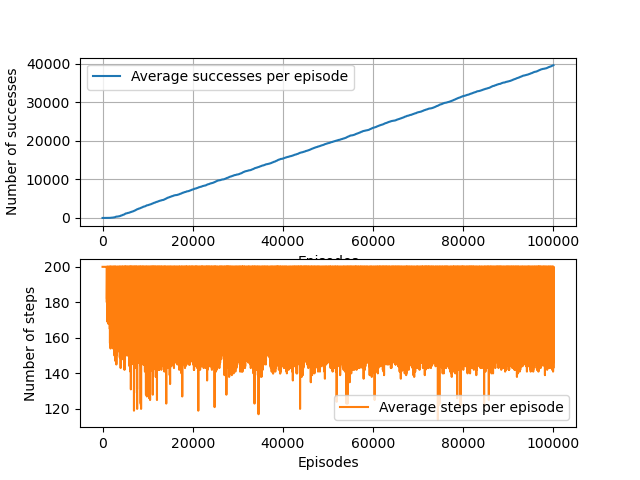
\includegraphics[width=0.8 \textwidth]{images/document/repeated_training_investigation_long.png}
\caption{Single evaluation over 100.000 episodes}
\label{fig:}
\end{figure}



\paragraph*{c) linear function approximation with RBF}

Instead of the simple identity feature vector $x$, we can use radial basis functions (RBF) to approximate the value function. The RBF is defined as
\begin{equation}
    \phi(x) = \exp\left(-\frac{1}{2\sigma^2}||x - \mu||^2\right)
\end{equation}
where $\mu$ is the center of the RBF, which is the current position of the mountain car and $\sigma$ the width, which is chosen to $\sigma=0.1$.

The learning curves for the RBF approximation are depicted in Figure \ref{fig:rbf}. The program is not optimized and therefore would take more than 16-fold time to run, than the single optimizer, even when flooring the value of the RBF below 0.01 to 0. Alternative approaches could be implemented by avoiding the back transformation to the discretized state-aggregation.

\begin{figure}[H]
\centering
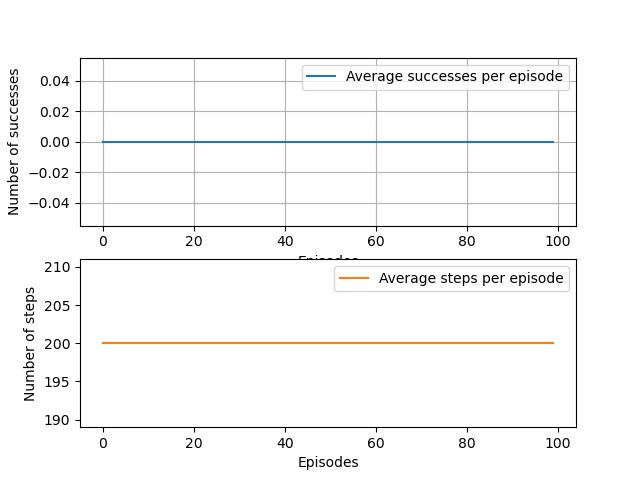
\includegraphics[width=0.8\textwidth]{images/document/repeated_training_investigation_rbf.png}
\caption{Learning curves for RBF approximation}
\label{fig:rbf}
\end{figure}
\end{document}













